\documentclass{article}

\usepackage{nonotation}
\usepackage{amssymb}
\usepackage{mathpazo}

\PassOptionsToPackage{hyphens}{url}
\usepackage{hyperref}

\hypersetup{
    colorlinks,
    linkcolor       = {red!70!black},
    citecolor       = {blue!50!black},
    urlcolor        = {blue!80!black}
}

% Hyperlink dingbat
\usepackage{pifont} 
\newcommand{\linkicon}{\ding{226}}

\usepackage{listings}
%\usepackage{inconsolata}
\lstdefinestyle{posh}
{
    backgroundcolor=\color{white},
    basicstyle=\scriptsize\color{black}\ttfamily
}

\title{Report --- PhaseKing statistical model check}
\author{Andrea Proietto}

\begin{document}
    \maketitle


    \section{Objective}

    This report is about an actual software implementing the \emph{Phase-King} consensus protocol; the objective of the former is to verify the software's correctness by means of a specific method of statistical model checking, that is \emph{Hypothesis testing}.

    \subsection{Statistical model checking}

    To model a system's successes and failures at a most coarse and generalized level, Bernoulli random variables can be used. Let $S$ be such variable, and say that $S = 1$ expresses that the system has failed, and $S = 0$ otherwise. Since it is unknown how likely the system will fail \emph{a priori}, a tentative estimate for the probability of failure is defined in $\varepsilon$; the goal then becomes to prove that a system failure occurs with no more probability than $\varepsilon$:

    \[
        \Pr[S = 1] < \varepsilon
    \]

    Analogously, the objective can be to disprove the contrary, which is that a failure is at least as likely to happen than the established threshold $\varepsilon$:

    \[
        \Pr[S = 1] \geq \varepsilon
    \]

    % \footnote{In the PhaseKing case, no relationship is present across single runs, therefore the runs' results are independent of each other. In a general case, the system state across runs does factor in choosing an input that maximizes failure probability}
    This last statement will be the \emph{hypothesis} that this model checking method will want to disprove. The main idea is to run the system multiple times, each time with random independent inputs, until either a failure is encountered, or a run count $N$ established beforehand is reached. The multiple runs do make for a geometric random variable $X$ grounded on the original variable $S$, which represents how many runs are needed before the system fails.

    Going further with the failure hunting mindset, the method ideally aims to disprove that a failure is guaranteed to happen in the $N$ runs:
    
    \[
        \Pr[X \leq N \knowing \Pr[S = 1] \geq \varepsilon] = 1
    \]

    And this arguably can be verified if $N$ is infinite; to keep things practical, the method settles for an arbitrarily large $N$, and transforms the no-failure guarantee into a high probability of success regulated by a \emph{confidence factor} $\delta$:
    
    \[
        \Pr[X \leq N \knowing \Pr[S = 1] \geq \varepsilon] \geq 1 - \delta
    \]

    This is finally the whole statement that the method wants to disprove: if after $N$ runs the system doesn't fail, then then a hypothetical failure is very unlikely to happen, regulated by the values of $\varepsilon$ and $\delta$:

    \[
        \Pr[X > N \knowing \Pr[S = 1] \geq \varepsilon] < \delta
    \]
    
    The number of runs was introduced arbitrarily, but can be computed once both $\varepsilon$ and $\delta$ are chosen:

    \[
        N = \frac{\log \delta}{\log (1 - \varepsilon)}
    \]
    
    \section{Implementation overview}
    
    \begin{figure}[ht]
        \centering
        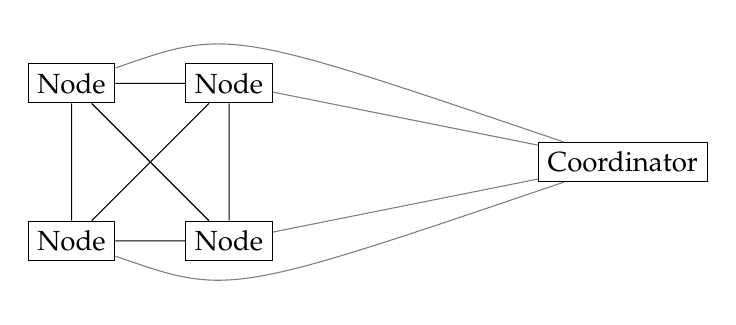
\begin{tikzpicture}
            \draw
                (0, 0) node (a) [draw, rectangle] {Node}
                (2, 0) node (b) [draw, rectangle] {Node}
                (0, 2) node (c) [draw, rectangle] {Node}
                (2, 2) node (d) [draw, rectangle] {Node}

                (7, 1) node (coord) [draw, rectangle] {Coordinator}

                (a) -- (b)
                (a) -- (c)
                (a) -- (d)
                (b) -- (c)
                (b) -- (d)
                (c) -- (d)
            ;

            \draw[color = gray]
                (b) -- (coord)
                (d) -- (coord)
                (a) .. controls (2, -0.7) .. (coord)
                (c) .. controls (2, 2.7) .. (coord)
            ;

        \end{tikzpicture}
        \caption{An instance of the complete system with 4 nodes participating in the Phase-King protocol}
        \label{fig:pk4ex}
    \end{figure}
    
    The whole system, along with the controlling logic, is implemented by means of Docker containers built from the OpenJDK15 image. The protocol itself is realized by a set of containers called \emph{nodes}, of which the shared source code is \texttt{Node.java}. The nodes are controlled by an additional container called the \emph{Coordinator}, and its source code is \texttt{Coordinator.java}. An example of the system is depicted in figure \ref{fig:pk4ex}, where the protocol implementation is tested on four nodes.
    
    The whole system is runnable from command-line by issuing two Docker commands, the first being necessary only on first run or parameter changes:

    \begin{lstlisting}[style=posh]
        > docker-compose build
        > docker-compose up
    \end{lstlisting}

    The parameters intended for tuning are in the file \texttt{.env}; of relevance are \texttt{PERC\_SUCCESS}, which is equivalent to $(1 - \varepsilon) / 100$, and \texttt{CONFIDENCE} which is $\delta$. Notably, the number of nodes \texttt{NODE\_COUNT} can be tuned too.

    
    \subsection{The protocol}

    The protocol implementation follows closely the definition in \cite{kshe08},\footnote{\linkicon \href
    {http://wwwusers.di.uniroma1.it/~stefa/Distributed_Systems/Schedule_files/consensus.pdf}
    {\textsf{``Consensus --- Distributed Systems course material, La Sapienza''}}} of which a sketch for node behaviour is reported here:

    \begin{enumerate}
        \item The node is assigned a unique identifier $i$ from the range $(1, n)$, where $n$ is the number of nodes;
        
        \item It then picks an initial binary value $v_i$, on which all nodes must agree upon at the end of protocol execution;

        \item For each phase $p$ from $1$ to $n/4 + 1$, where $n$ is the number of nodes:

        \begin{enumerate}
            \item[\textsc{Round 1}.] Broadcast $v_i$ to all peers, then receive all other $v_j$ from them, and compute which binary value $m_i$ has the majority among all values, and how much is the majority $c$;
            \item[\textsc{Round 2}.] The node decides if it's the Phase King in the current phase ($p = i$):

            \begin{itemize}
                \item if so, then it broadcasts its own value $m_i$ to all peers, which in turn will serve as tiebreaker to them; furthermore, $m_i$ becomes the next $v_i$ for the new phase;
                \item otherwise, the next $v_i$ will be either $b_i$ or the tiebreaker from the King, depending on whether the majority $c$ crosses a certain threshold ($c > n / 2 + f$).
            \end{itemize}

        \end{enumerate}

    \end{enumerate}


    \subsection{The control mechanism}

    The coordinator is responsible for:

    \begin{itemize}
        \item Ensuring that all nodes are connected;
        \item Deciding the behaviour for each node, either honest or byzantine;
        \item Synchronizing the nodes' status and phases;
        \item Enforcing statistical model checking on the protocol implementation, and reporting the results.
    \end{itemize}

    When launched, the coordinator will compute the number of runs required to enforce hypothesis testing, and when finished, will report whether the process has been successful or not. Other than that, the coordinator does not partake in the Phase-King protocol in any way. 

    \pagebreak

    \section{Results and the future}

    The software has been run with varying values for the number of nodes, lower bound for probability of success, and confidence factor, with the results shown in table \ref{table:results}. Each check also reports the number of tests performed in order to enforce the thesis of hypothesis testing.

    \begin{table}[ht]
        \caption{Model checking results}
        \centering
        \vbox{}
        \begin{tabular}{cc|cc|c}
            \hline\hline\noalign{\smallskip}
            \# Nodes & \shortstack[c]{Phases per \\ session} & \shortstack[c]{Success \\ guarantee} & \shortstack[c]{Confidence \\ factor} & \shortstack[c]{Outcome \\ (\# Tests)} \\[0.5ex]
            \hline\noalign{\smallskip}
            10 & 2  & 99\% & 0.001 & \checkmark(688) \\
            -- & -- & 99\% & 0.0001 & \checkmark(917) \\
            -- & -- & 99.9\% & 0.001 & \checkmark(6905) \\
            -- & -- & 99.9\% & 0.0001 & \checkmark(9206) \\
            15 & 3  & 99\% & 0.001 & \checkmark(688) \\
            -- & -- & 99\% & 0.0001 & \checkmark(917) \\
            -- & -- & 99.9\% & 0.001 & \checkmark(6905) \\
            -- & -- & 99.9\% & 0.0001 & \checkmark(9206) \\
            30 & 7  & 99\% & 0.001 & \checkmark(688) \\
            -- & -- & 99\% & 0.0001 & \checkmark(917) \\
            -- & -- & 99.9\% & 0.001 & \checkmark(6905) \\
            -- & -- & 99.9\% & 0.0001 & \checkmark(9206) \\[1ex]
            \hline
        \end{tabular}
        \label{table:results}
    \end{table}

    So far, all tests are passed successfully, including the last and most demanding test one, which guarantees that a network of 30 nodes reaches consensus with a reliability of 99.9\% and a confidence factor of $10^{-4}$.
    
    Tests with stricter parameters have not been performed due to current technical limitations, and the assumption that these results are good enough as is. With more computational power, and the use of Docker's swarm functionality, it is expected that the parameters can be brought to extreme values, while still guaranteeing the software's correctness.


    \begin{thebibliography}{9}
        \bibitem{kshe08}
            \textsc{A. D. Kshemkalyani, M. Singhal},
            \textit{Distributed Computing: Principles, Algorithms, and Systems}, page 527,
            Cambridge University Press, 2008

    \end{thebibliography}

\end{document}